\documentclass[11pt,a4paper]{article}
\usepackage[utf8]{inputenc}
\usepackage[T1]{fontenc}


\usepackage{physics}
\usepackage{amsmath}
\usepackage{tikz}
\usepackage{mathdots}
\usepackage{yhmath}
\usepackage{cancel}
\usepackage{color}
\usepackage{siunitx}
\usepackage{array}
\usepackage{multirow}
\usepackage{amssymb}
\usepackage{gensymb}
\usepackage{tabularx}
\usepackage{extarrows}
\usepackage{booktabs}
\usetikzlibrary{fadings}
\usetikzlibrary{patterns}
\usetikzlibrary{shadows.blur}
\usetikzlibrary{shapes}



\usepackage[left=2.00cm, right=2.00cm]{geometry}
\title{Coordinates in Spring Problems}
\author{Ali Fele Paranj}
\begin{document}
	
\maketitle
\section{Coordinates in spring problems}
Different coordinates to solve spring problems, despite they are very simple, were always confusing for me. Here in this note I am going to summarize them for my future references.
\subsection{One String, Two Masses}
Let's start with a spring and two connected masses to its ends.
\begin{figure}[h!]
\tikzset{every picture/.style={line width=0.75pt}} %set default line width to 0.75pt        
\centering
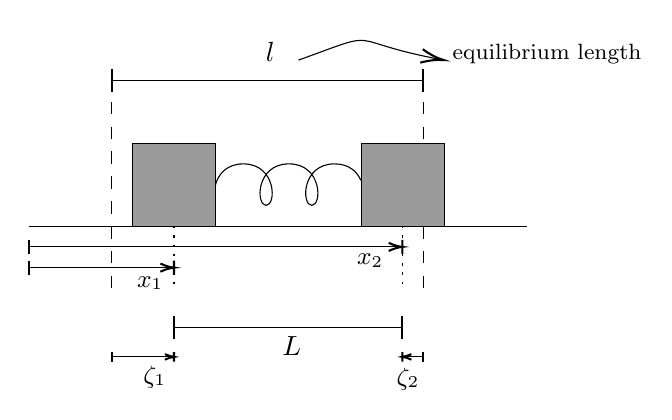
\begin{tikzpicture}[x=0.75pt,y=0.75pt,yscale=-1,xscale=1]
	%uncomment if require: \path (0,300); %set diagram left start at 0, and has height of 300
	
	%Straight Lines [id:da49024415917117725] 
	\draw  [dash pattern={on 4.5pt off 4.5pt}]  (260,40) -- (260,130) ;
	%Straight Lines [id:da17002373577888874] 
	\draw  [dash pattern={on 0.84pt off 2.51pt}]  (140,100) -- (140,130) ;
	%Straight Lines [id:da3622966258850706] 
	\draw    (70,100) -- (310,100) ;
	%Shape: Square [id:dp7274505039801786] 
	\draw  [fill={rgb, 255:red, 155; green, 155; blue, 155 }  ,fill opacity=1 ] (120,60) -- (160,60) -- (160,100) -- (120,100) -- cycle ;
	%Shape: Square [id:dp1418594952139698] 
	\draw  [fill={rgb, 255:red, 155; green, 155; blue, 155 }  ,fill opacity=1 ] (230.5,60) -- (270.5,60) -- (270.5,100) -- (230.5,100) -- cycle ;
	%Shape: Spring [id:dp8678123163902718] 
	\draw   (160,80) .. controls (161.38,75) and (165.38,70) .. (173.38,70) .. controls (189.38,70) and (189.38,90) .. (184.38,90) .. controls (179.38,90) and (179.38,70) .. (195.38,70) .. controls (211.38,70) and (211.38,90) .. (206.38,90) .. controls (201.38,90) and (201.38,70) .. (217.38,70) .. controls (224.24,70) and (228.16,73.68) .. (230,77.88) ;
	%Straight Lines [id:da7059608722848922] 
	\draw  [dash pattern={on 0.84pt off 2.51pt}]  (250,100) -- (250,130) ;
	%Straight Lines [id:da5463813672950899] 
	\draw  [dash pattern={on 4.5pt off 4.5pt}]  (110,40) -- (110,130) ;
	%Straight Lines [id:da7496363746635586] 
	\draw    (110,30) -- (260,30) ;
	\draw [shift={(260,30)}, rotate = 180] [color={rgb, 255:red, 0; green, 0; blue, 0 }  ][line width=0.75]    (0,5.59) -- (0,-5.59)   ;
	\draw [shift={(110,30)}, rotate = 180] [color={rgb, 255:red, 0; green, 0; blue, 0 }  ][line width=0.75]    (0,5.59) -- (0,-5.59)   ;
	%Straight Lines [id:da9436728329184318] 
	\draw    (140,149) -- (250,149) ;
	\draw [shift={(250,149)}, rotate = 180] [color={rgb, 255:red, 0; green, 0; blue, 0 }  ][line width=0.75]    (0,5.59) -- (0,-5.59)   ;
	\draw [shift={(140,149)}, rotate = 180] [color={rgb, 255:red, 0; green, 0; blue, 0 }  ][line width=0.75]    (0,5.59) -- (0,-5.59)   ;
	%Curve Lines [id:da5969328405316103] 
	\draw    (200,20) .. controls (242.57,4.65) and (219.47,10.38) .. (268.49,19.72) ;
	\draw [shift={(270,20)}, rotate = 190.55] [color={rgb, 255:red, 0; green, 0; blue, 0 }  ][line width=0.75]    (10.93,-3.29) .. controls (6.95,-1.4) and (3.31,-0.3) .. (0,0) .. controls (3.31,0.3) and (6.95,1.4) .. (10.93,3.29)   ;
	%Straight Lines [id:da6584585700602277] 
	\draw    (110,163) -- (140,163) ;
	\draw [shift={(140,163)}, rotate = 180] [color={rgb, 255:red, 0; green, 0; blue, 0 }  ][line width=0.75]    (0,2.24) -- (0,-2.24)(4.37,-1.32) .. controls (2.78,-0.56) and (1.32,-0.12) .. (0,0) .. controls (1.32,0.12) and (2.78,0.56) .. (4.37,1.32)   ;
	\draw [shift={(110,163)}, rotate = 180] [color={rgb, 255:red, 0; green, 0; blue, 0 }  ][line width=0.75]    (0,2.24) -- (0,-2.24)   ;
	%Straight Lines [id:da23707744688318644] 
	\draw    (250,163) -- (260,163) ;
	\draw [shift={(260,163)}, rotate = 180] [color={rgb, 255:red, 0; green, 0; blue, 0 }  ][line width=0.75]    (0,2.24) -- (0,-2.24)   ;
	\draw [shift={(250,163)}, rotate = 0] [color={rgb, 255:red, 0; green, 0; blue, 0 }  ][line width=0.75]    (0,2.24) -- (0,-2.24)(4.37,-1.32) .. controls (2.78,-0.56) and (1.32,-0.12) .. (0,0) .. controls (1.32,0.12) and (2.78,0.56) .. (4.37,1.32)   ;
	%Straight Lines [id:da8470667367671667] 
	\draw    (70,110) -- (250,110) ;
	\draw [shift={(250,110)}, rotate = 180] [color={rgb, 255:red, 0; green, 0; blue, 0 }  ][line width=0.75]    (0,3.35) -- (0,-3.35)(6.56,-1.97) .. controls (4.17,-0.84) and (1.99,-0.18) .. (0,0) .. controls (1.99,0.18) and (4.17,0.84) .. (6.56,1.97)   ;
	\draw [shift={(70,110)}, rotate = 180] [color={rgb, 255:red, 0; green, 0; blue, 0 }  ][line width=0.75]    (0,3.35) -- (0,-3.35)   ;
	%Straight Lines [id:da4986049190957611] 
	\draw    (70,120) -- (140,120) ;
	\draw [shift={(140,120)}, rotate = 180] [color={rgb, 255:red, 0; green, 0; blue, 0 }  ][line width=0.75]    (0,3.35) -- (0,-3.35)(6.56,-1.97) .. controls (4.17,-0.84) and (1.99,-0.18) .. (0,0) .. controls (1.99,0.18) and (4.17,0.84) .. (6.56,1.97)   ;
	\draw [shift={(70,120)}, rotate = 180] [color={rgb, 255:red, 0; green, 0; blue, 0 }  ][line width=0.75]    (0,3.35) -- (0,-3.35)   ;
	
	% Text Node
	\draw (183,10) node [anchor=north west][inner sep=0.75pt]   [align=left] {$\displaystyle l$};
	% Text Node
	\draw (121,123) node [anchor=north west][inner sep=0.75pt]  [font=\small] [align=left] {$\displaystyle x_{1}$};
	% Text Node
	\draw (227,112) node [anchor=north west][inner sep=0.75pt]  [font=\small] [align=left] {$\displaystyle x_{2}$};
	% Text Node
	\draw (191,152) node [anchor=north west][inner sep=0.75pt]   [align=left] {$\displaystyle L$};
	% Text Node
	\draw (273,11) node [anchor=north west][inner sep=0.75pt]   [align=left] {{\footnotesize equilibrium length}};
	% Text Node
	\draw (124,166) node [anchor=north west][inner sep=0.75pt]  [font=\small] [align=left] {$\displaystyle \zeta _{1}$};
	% Text Node
	\draw (246,167) node [anchor=north west][inner sep=0.75pt]  [font=\small] [align=left] {$\displaystyle \zeta _{2}$};
\end{tikzpicture}
\end{figure}

The most simple way to write the equations of motion is to use the coordinates $x_1$, and $x_2$. Also note that $l$ represents the length of spring that corresponds to its equilibrium size (meaning that in that length, the spring is not under compression or under tension). The variable $L$ represents the spacing between two masses. With these variables in hand we can write the equations of motions
\begin{align*}
	F_1 = k (x_2-x_1-l), \\
	F_2 =- k (x_2 - x_1 - l).
\end{align*}
By imagining some cases, we can argue that the above equations are correct for the forces. As an example, suppose that both masses are at equilibrium. Then $x_2 - x_1 - l$ will be zero, thus the force on mass 1 and (mass 2) will be zero. Now imagine that $x_2 - x_1 - l$ is negative. This means that the spring is under contraction thus exerts force to mass one in the negative direction which is also clear from the equations for the forces. Similarly, assume that $x_2 - x_1 - l$ is positive which indicates that the spring is under tension, thus exerts a force to the mass 1 in the positive direction.

By a simple change of variable, we can write the force equations in a more clean way. For this purpose, we will use the variables $\zeta_1$ and $\zeta_{2}$. From figure it is clear that
\[ x_1 - \zeta_{1} + l + \zeta_{2} = x_2. \]
By rearranging the terms we can write:
\[ \zeta_{2} - \zeta_{1} = x_2 - x_1 - l. \] 
Now we can substitute this equation in the old equations of motions. Then we will have:
\begin{align*}
	F_1 &= k(\zeta_{2} - \zeta_{1}), \\
	F_2 &= -k(\zeta_{2} - \zeta_{1}).
\end{align*}

By testing some cases, we can make sure that the equations are correct. For example, imagine the case in which mass 1 is deviated from the equilibrium point to the right. Then $\zeta_{1}>0$ and $\zeta_{2}=0$. Then the equations of motions correctly results in the force to mass 1 in the negative direction.

\subsection{Three Springs, Two Masses}
We can do the same for any number of springs and masses. In this section we are going to write down the force equations for the masses $m_1$ and $m_2$. Similar to the above example, we can write the force equations in terms of $x_1$ and $x_2$.


\begin{figure}[h!]
	\centering
	\tikzset{every picture/.style={line width=0.75pt}} %set default line width to 0.75pt        
	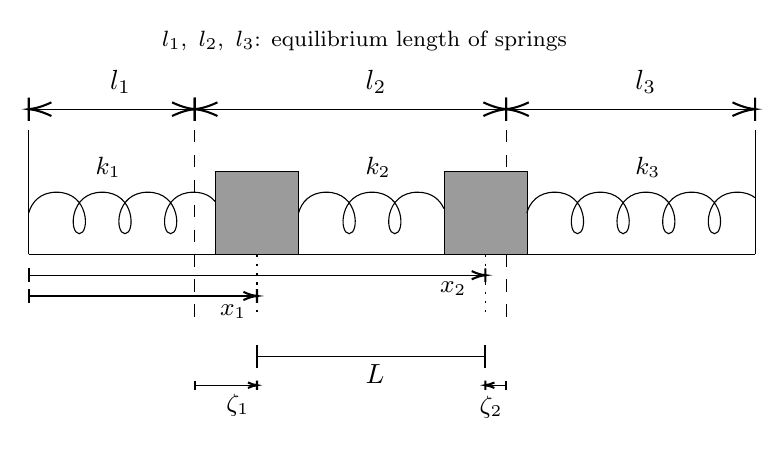
\begin{tikzpicture}[x=0.75pt,y=0.75pt,yscale=-1,xscale=1]
		%uncomment if require: \path (0,300); %set diagram left start at 0, and has height of 300
		
		%Straight Lines [id:da7182131922856716] 
		\draw  [dash pattern={on 4.5pt off 4.5pt}]  (300,90) -- (300,180) ;
		%Straight Lines [id:da7152276308205743] 
		\draw  [dash pattern={on 0.84pt off 2.51pt}]  (180,150) -- (180,180) ;
		%Straight Lines [id:da055077321297104964] 
		\draw    (70,150) -- (420,150) ;
		%Shape: Square [id:dp9865563239692134] 
		\draw  [fill={rgb, 255:red, 155; green, 155; blue, 155 }  ,fill opacity=1 ] (160,110) -- (200,110) -- (200,150) -- (160,150) -- cycle ;
		%Shape: Square [id:dp7735995299256013] 
		\draw  [fill={rgb, 255:red, 155; green, 155; blue, 155 }  ,fill opacity=1 ] (270.5,110) -- (310.5,110) -- (310.5,150) -- (270.5,150) -- cycle ;
		%Shape: Spring [id:dp8199474715736716] 
		\draw   (200,130) .. controls (201.38,125) and (205.38,120) .. (213.38,120) .. controls (229.38,120) and (229.38,140) .. (224.38,140) .. controls (219.38,140) and (219.38,120) .. (235.38,120) .. controls (251.38,120) and (251.38,140) .. (246.38,140) .. controls (241.38,140) and (241.38,120) .. (257.38,120) .. controls (264.24,120) and (268.16,123.68) .. (270,127.88) ;
		%Straight Lines [id:da6661168026696984] 
		\draw  [dash pattern={on 0.84pt off 2.51pt}]  (290,150) -- (290,180) ;
		%Straight Lines [id:da41121793639305126] 
		\draw  [dash pattern={on 4.5pt off 4.5pt}]  (150,90) -- (150,180) ;
		%Straight Lines [id:da4580757275819549] 
		\draw    (150,80) -- (300,80) ;
		\draw [shift={(300,80)}, rotate = 180] [color={rgb, 255:red, 0; green, 0; blue, 0 }  ][line width=0.75]    (0,5.59) -- (0,-5.59)(10.93,-3.29) .. controls (6.95,-1.4) and (3.31,-0.3) .. (0,0) .. controls (3.31,0.3) and (6.95,1.4) .. (10.93,3.29)   ;
		\draw [shift={(150,80)}, rotate = 0] [color={rgb, 255:red, 0; green, 0; blue, 0 }  ][line width=0.75]    (0,5.59) -- (0,-5.59)(10.93,-3.29) .. controls (6.95,-1.4) and (3.31,-0.3) .. (0,0) .. controls (3.31,0.3) and (6.95,1.4) .. (10.93,3.29)   ;
		%Straight Lines [id:da44512646549656787] 
		\draw    (180,199) -- (290,199) ;
		\draw [shift={(290,199)}, rotate = 180] [color={rgb, 255:red, 0; green, 0; blue, 0 }  ][line width=0.75]    (0,5.59) -- (0,-5.59)   ;
		\draw [shift={(180,199)}, rotate = 180] [color={rgb, 255:red, 0; green, 0; blue, 0 }  ][line width=0.75]    (0,5.59) -- (0,-5.59)   ;
		%Straight Lines [id:da01808433905476181] 
		\draw    (150,213) -- (180,213) ;
		\draw [shift={(180,213)}, rotate = 180] [color={rgb, 255:red, 0; green, 0; blue, 0 }  ][line width=0.75]    (0,2.24) -- (0,-2.24)(4.37,-1.32) .. controls (2.78,-0.56) and (1.32,-0.12) .. (0,0) .. controls (1.32,0.12) and (2.78,0.56) .. (4.37,1.32)   ;
		\draw [shift={(150,213)}, rotate = 180] [color={rgb, 255:red, 0; green, 0; blue, 0 }  ][line width=0.75]    (0,2.24) -- (0,-2.24)   ;
		%Straight Lines [id:da08608425111338547] 
		\draw    (290,213) -- (300,213) ;
		\draw [shift={(300,213)}, rotate = 180] [color={rgb, 255:red, 0; green, 0; blue, 0 }  ][line width=0.75]    (0,2.24) -- (0,-2.24)   ;
		\draw [shift={(290,213)}, rotate = 0] [color={rgb, 255:red, 0; green, 0; blue, 0 }  ][line width=0.75]    (0,2.24) -- (0,-2.24)(4.37,-1.32) .. controls (2.78,-0.56) and (1.32,-0.12) .. (0,0) .. controls (1.32,0.12) and (2.78,0.56) .. (4.37,1.32)   ;
		%Straight Lines [id:da7921489292693746] 
		\draw    (70,160) -- (290,160) ;
		\draw [shift={(290,160)}, rotate = 180] [color={rgb, 255:red, 0; green, 0; blue, 0 }  ][line width=0.75]    (0,3.35) -- (0,-3.35)(6.56,-1.97) .. controls (4.17,-0.84) and (1.99,-0.18) .. (0,0) .. controls (1.99,0.18) and (4.17,0.84) .. (6.56,1.97)   ;
		\draw [shift={(70,160)}, rotate = 180] [color={rgb, 255:red, 0; green, 0; blue, 0 }  ][line width=0.75]    (0,3.35) -- (0,-3.35)   ;
		%Straight Lines [id:da9054293907421247] 
		\draw    (70,170) -- (180,170) ;
		\draw [shift={(180,170)}, rotate = 180] [color={rgb, 255:red, 0; green, 0; blue, 0 }  ][line width=0.75]    (0,3.35) -- (0,-3.35)(6.56,-1.97) .. controls (4.17,-0.84) and (1.99,-0.18) .. (0,0) .. controls (1.99,0.18) and (4.17,0.84) .. (6.56,1.97)   ;
		\draw [shift={(70,170)}, rotate = 180] [color={rgb, 255:red, 0; green, 0; blue, 0 }  ][line width=0.75]    (0,3.35) -- (0,-3.35)   ;
		%Shape: Spring [id:dp6980397929340345] 
		\draw   (70,130) .. controls (71.38,125) and (75.38,120) .. (83.38,120) .. controls (99.38,120) and (99.38,140) .. (94.38,140) .. controls (89.38,140) and (89.38,120) .. (105.38,120) .. controls (121.38,120) and (121.38,140) .. (116.38,140) .. controls (111.38,140) and (111.38,120) .. (127.38,120) .. controls (143.38,120) and (143.38,140) .. (138.38,140) .. controls (133.38,140) and (133.38,120) .. (149.38,120) .. controls (154.36,120) and (157.79,121.94) .. (160,124.61) ;
		%Shape: Spring [id:dp9185073736887013] 
		\draw   (310,130) .. controls (311.38,125) and (315.38,120) .. (323.38,120) .. controls (339.38,120) and (339.38,140) .. (334.38,140) .. controls (329.38,140) and (329.38,120) .. (345.38,120) .. controls (361.38,120) and (361.38,140) .. (356.38,140) .. controls (351.38,140) and (351.38,120) .. (367.38,120) .. controls (383.38,120) and (383.38,140) .. (378.38,140) .. controls (373.38,140) and (373.38,120) .. (389.38,120) .. controls (405.38,120) and (405.38,140) .. (400.38,140) .. controls (395.38,140) and (395.38,120) .. (411.38,120) .. controls (415.05,120) and (417.88,121.05) .. (420,122.68) ;
		%Straight Lines [id:da567648501513367] 
		\draw    (70,150) -- (70,90) ;
		%Straight Lines [id:da09550724549228651] 
		\draw    (420,150) -- (420,90) ;
		%Straight Lines [id:da016629326871508532] 
		\draw    (70,80) -- (150,80) ;
		\draw [shift={(150,80)}, rotate = 180] [color={rgb, 255:red, 0; green, 0; blue, 0 }  ][line width=0.75]    (0,5.59) -- (0,-5.59)(10.93,-3.29) .. controls (6.95,-1.4) and (3.31,-0.3) .. (0,0) .. controls (3.31,0.3) and (6.95,1.4) .. (10.93,3.29)   ;
		\draw [shift={(70,80)}, rotate = 0] [color={rgb, 255:red, 0; green, 0; blue, 0 }  ][line width=0.75]    (0,5.59) -- (0,-5.59)(10.93,-3.29) .. controls (6.95,-1.4) and (3.31,-0.3) .. (0,0) .. controls (3.31,0.3) and (6.95,1.4) .. (10.93,3.29)   ;
		%Straight Lines [id:da07124946774692154] 
		\draw    (300,80) -- (311,80) -- (420,80) ;
		\draw [shift={(420,80)}, rotate = 180] [color={rgb, 255:red, 0; green, 0; blue, 0 }  ][line width=0.75]    (0,5.59) -- (0,-5.59)(10.93,-3.29) .. controls (6.95,-1.4) and (3.31,-0.3) .. (0,0) .. controls (3.31,0.3) and (6.95,1.4) .. (10.93,3.29)   ;
		\draw [shift={(300,80)}, rotate = 0] [color={rgb, 255:red, 0; green, 0; blue, 0 }  ][line width=0.75]    (0,5.59) -- (0,-5.59)(10.93,-3.29) .. controls (6.95,-1.4) and (3.31,-0.3) .. (0,0) .. controls (3.31,0.3) and (6.95,1.4) .. (10.93,3.29)   ;
		
		% Text Node
		\draw (108,60) node [anchor=north west][inner sep=0.75pt]   [align=left] {$\displaystyle l_{1}$};
		% Text Node
		\draw (161,173) node [anchor=north west][inner sep=0.75pt]  [font=\small] [align=left] {$\displaystyle x_{1}$};
		% Text Node
		\draw (267,162) node [anchor=north west][inner sep=0.75pt]  [font=\small] [align=left] {$\displaystyle x_{2}$};
		% Text Node
		\draw (231,202) node [anchor=north west][inner sep=0.75pt]   [align=left] {$\displaystyle L$};
		% Text Node
		\draw (133,41) node [anchor=north west][inner sep=0.75pt]   [align=left] {{\footnotesize $\displaystyle l_{1} ,\ l_{2} ,\ l_{3}$: equilibrium length of springs}};
		% Text Node
		\draw (164,216) node [anchor=north west][inner sep=0.75pt]  [font=\small] [align=left] {$\displaystyle \zeta _{1}$};
		% Text Node
		\draw (286,217) node [anchor=north west][inner sep=0.75pt]  [font=\small] [align=left] {$\displaystyle \zeta _{2}$};
		% Text Node
		\draw (101,102) node [anchor=north west][inner sep=0.75pt]  [font=\small] [align=left] {$\displaystyle k_{1}$};
		% Text Node
		\draw (231,102) node [anchor=north west][inner sep=0.75pt]  [font=\small] [align=left] {$\displaystyle k_{2}$};
		% Text Node
		\draw (361,102) node [anchor=north west][inner sep=0.75pt]  [font=\small] [align=left] {$\displaystyle k_{3}$};
		% Text Node
		\draw (231,60) node [anchor=north west][inner sep=0.75pt]   [align=left] {$\displaystyle l_{2}$};
		% Text Node
		\draw (361,60) node [anchor=north west][inner sep=0.75pt]   [align=left] {$\displaystyle l_{3}$};
		
	\end{tikzpicture}
\end{figure}

From the figure above, it is clear that two springs exert force the mass $m_1$. The net force to mass 1 will be:
\[  F_1 = -k_1 (x_1 - l_1) + k_2 (x_2 - x_1 - l_2). \] In a similar way we can write down the equation of forces to mass 2 which will be:
\[  F_2 = -k_2 (x_2 - x_1 - l_2) - k_3 (x_2 - (l_1 + l_2)). \] The equations are not very clean and that is an indicator that we are not using the natural variables to describe the system. Like the previous example, we can write down the equations of motion using the variables $\zeta_{1}$ and $\zeta_{2}$. From figure, we can write:
\begin{align*}
	& \zeta_1 = x_1 - l_1, \\
	& x_2 - x_1 - l_2 = (l_1 + l_2 + \zeta_{2}) - (l_1 + \zeta_{1}) - l_2 = \zeta_{2} - \zeta_{1},\\
	& x_2 - (l_1 + l_2) = (l_1 + l_2 + \zeta_{2}) - (l_1 + l_2)  = \zeta_{2}.
\end{align*}
So the equation for forces can be written as:
\begin{align*}
	F_1 = - k_1 \zeta_1 + k_2 (\zeta_2 - \zeta_1) &= -(k_1 + k_2)\zeta_1 + k_2 \zeta_2, \\
	F_2 = -k_2 (\zeta_2 - \zeta_1) - k_3 \zeta_2 &= k_2 \zeta_1 - (k_2 + k_3) \zeta_2.
\end{align*}
 

\end{document}


